\section{Debug linux 内核的总结}
  \subsection{QEMU脚本}
  \begin{lstlisting}
    qemu-system-x86_64 -kernel ./linux/arch/x86_64/boot/bzImage -initrd \
                ../Download/busybox-1.36.1/_install/rootfs.img \
                -append "nokaslr console=ttyS0" -s -S -nographic
  \end{lstlisting}
 \begin{figure}[htbp]
  \begin{center}
  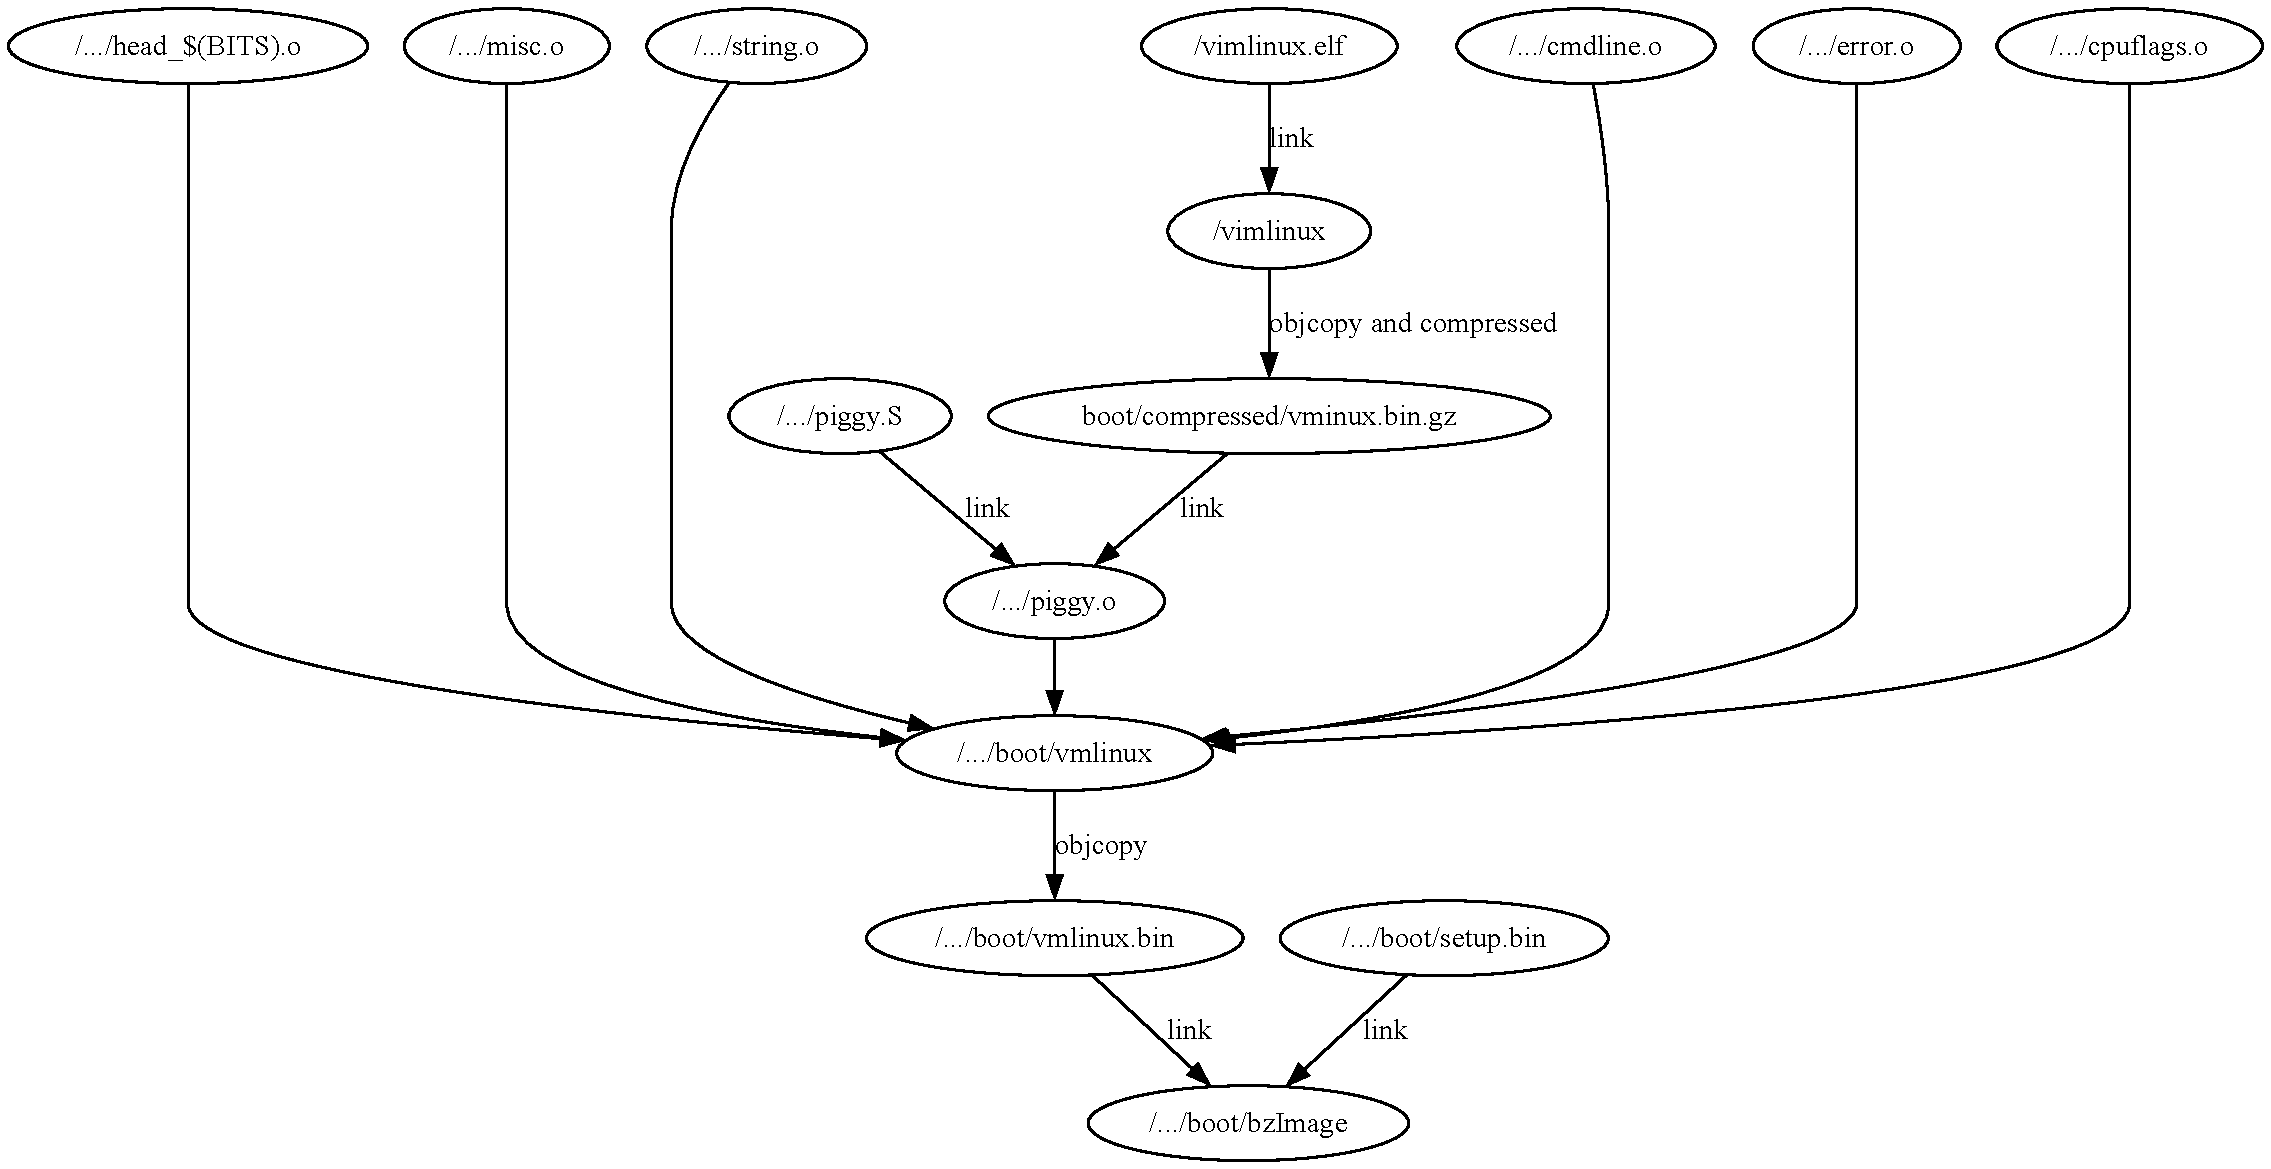
\includegraphics[width=0.95\textwidth]{Pictures/vmlinux_arch.pdf}
\end{center}
 \end{figure}
  \subsection{一些问题}
    \begin{itemize}
      \item 关于为什么在QEMU中进行debug无法在start\_kernel函数之前打断点?
      这里做如下解释:当镜像文件为zbImage时,镜像文件为压缩文件,QEMU在没有解压之前无法识别
      正确的函数符号与名称(加载符号文件的根目录下的vmlinux并没有setup和compressed内容),因此无法打断点
      \item  若需要直接debug vmlinux 文件(主文件),必须在内核编译配置时增加PVH,
      并且开启后在debug中会直接跳转的0x7c00的代码段中,由于没有引导程序,在0x7c00出死循环
      \item debug\quad 某可执行程序,程序是由gdb创建子进程,因而可以控制其运动
      \item gdbrun\quad 运行程序自动在main函数停止\quad b\quad filename:line\_number\quad 在某个人间的某一行打断点
      \item gdb\quad list 显示程序的行代码,注意main函数不一定在第0行,未执行的地方无法显示,debug可以和printf一起用
   \end{itemize}
    